\documentclass{article}
\usepackage{tikz}
\usetikzlibrary{shapes.geometric, arrows.meta, positioning}

\begin{document}

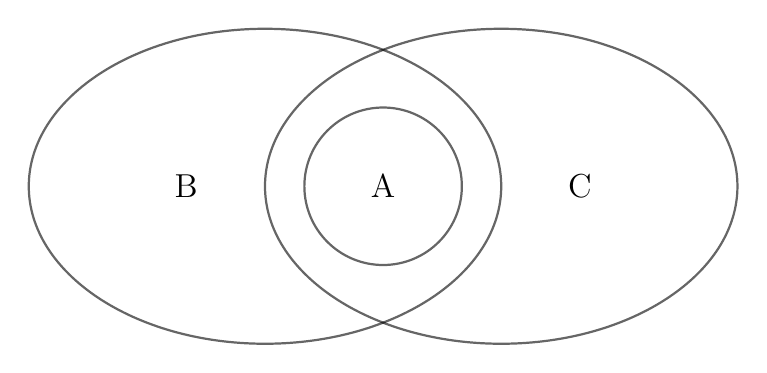
\begin{tikzpicture}[
    set/.style={
        ellipse, 
        draw=black, 
        thick, 
        minimum width=2cm, 
        minimum height=2cm,
        opacity=0.6
    },
    label/.style={font=\large, inner sep=2pt}
]

% 定义三个椭圆集合的位置
\node[set, minimum width = 6cm, minimum height = 4cm, label={[label]B}] (B) at (0,0) {};
\node[set, minimum width = 6cm, minimum height = 4cm, label={[label]C}] (C) at (3,0) {};
\node[set, label={[label]A}] (A) at (1.5,0) {};

% 添加公式标签
\node[label] at (1.5, 0) {A};
\node[label] at (-1, 0) {B};
\node[label] at (4, 0) {C};

\end{tikzpicture}

\end{document}